\documentclass[12pt,letterpaper]{article}
\usepackage[utf8]{inputenc}
\usepackage{float, xcolor}

%----- Configuración del estilo del documento------%
\usepackage{graphicx, fancyhdr, lastpage}
\usepackage{enumitem, pifont}
\usepackage[left=2cm,right=2cm,top=1.8cm,bottom=2.3cm]{geometry}

\pagestyle{fancy}
\fancyhf{}
\rfoot{\textit{Página \thepage \hspace{1pt} de \pageref{LastPage}}}

%------ Paquetes matemáticos básicos --------%
\usepackage{amsmath, amssymb, amsthm}

\begin{document}

%------ Encabezado -------- %
\begin{center}
\newcommand{\imp}{\rightarrow}
\newcommand{\vp}{\varphi}
  \begin{minipage}{3cm}
    \begin{center}
      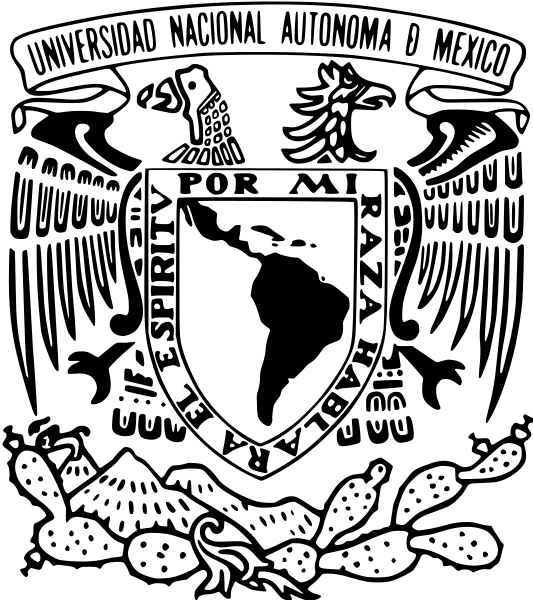
\includegraphics[height=3.4cm]{unam_logo.png}
    \end{center}
  \end{minipage}\hfill
  \begin{minipage}{10cm}
    \begin{center}
      \textbf{\Large Universidad Nacional Autónoma de México}\\[0.2cm]
      \textbf{\large Facultad de Ciencias}\\[0.2cm]
      \textbf{Organización y Arquitectura de Computadoras 2025-2}\\[0.4cm]
      \textbf{\Large Práctica 03}\\[0.1cm]
      \textbf{Docentes:}\\
      José Galaviz \hspace{1em} Ricardo Pérez \hspace{1em} Ximena Lezama\\[0.3cm]
      \textbf{Autores:}\\
      Fernanda Ramírez Juárez \quad Ianluck Rojo Peña\\[0.3cm]
      \textbf{Fecha de entrega:} Jueves 27 de febrero de 2025
    \end{center}
  \end{minipage}\hfill
  \begin{minipage}{3cm}
    \begin{center}
      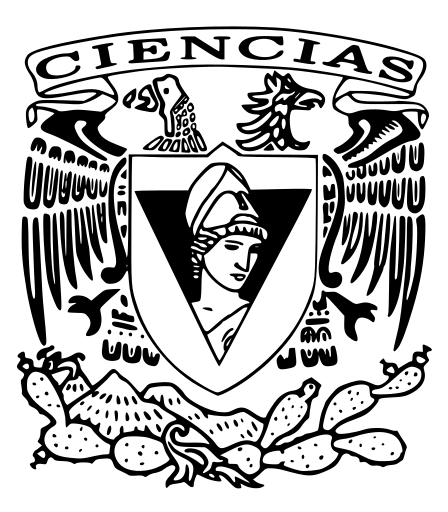
\includegraphics[height=3.4cm]{fc_logo.png}
    \end{center}
  \end{minipage}
\end{center}

\bigskip
\hrule height 0.1pt
\bigskip

%------ Contenido -------- %
\section*{Ejercicios.}

\begin{itemize}
\item Dada la siguiente tabla de verdad. Reducirla usando Mapas de Karnaugh, implementar el circuito resultante y contestar. ¿Que hace el circuito resultante?
  
  % -- Respuesta -- %
  \begin{figure}[H]
    \centering
      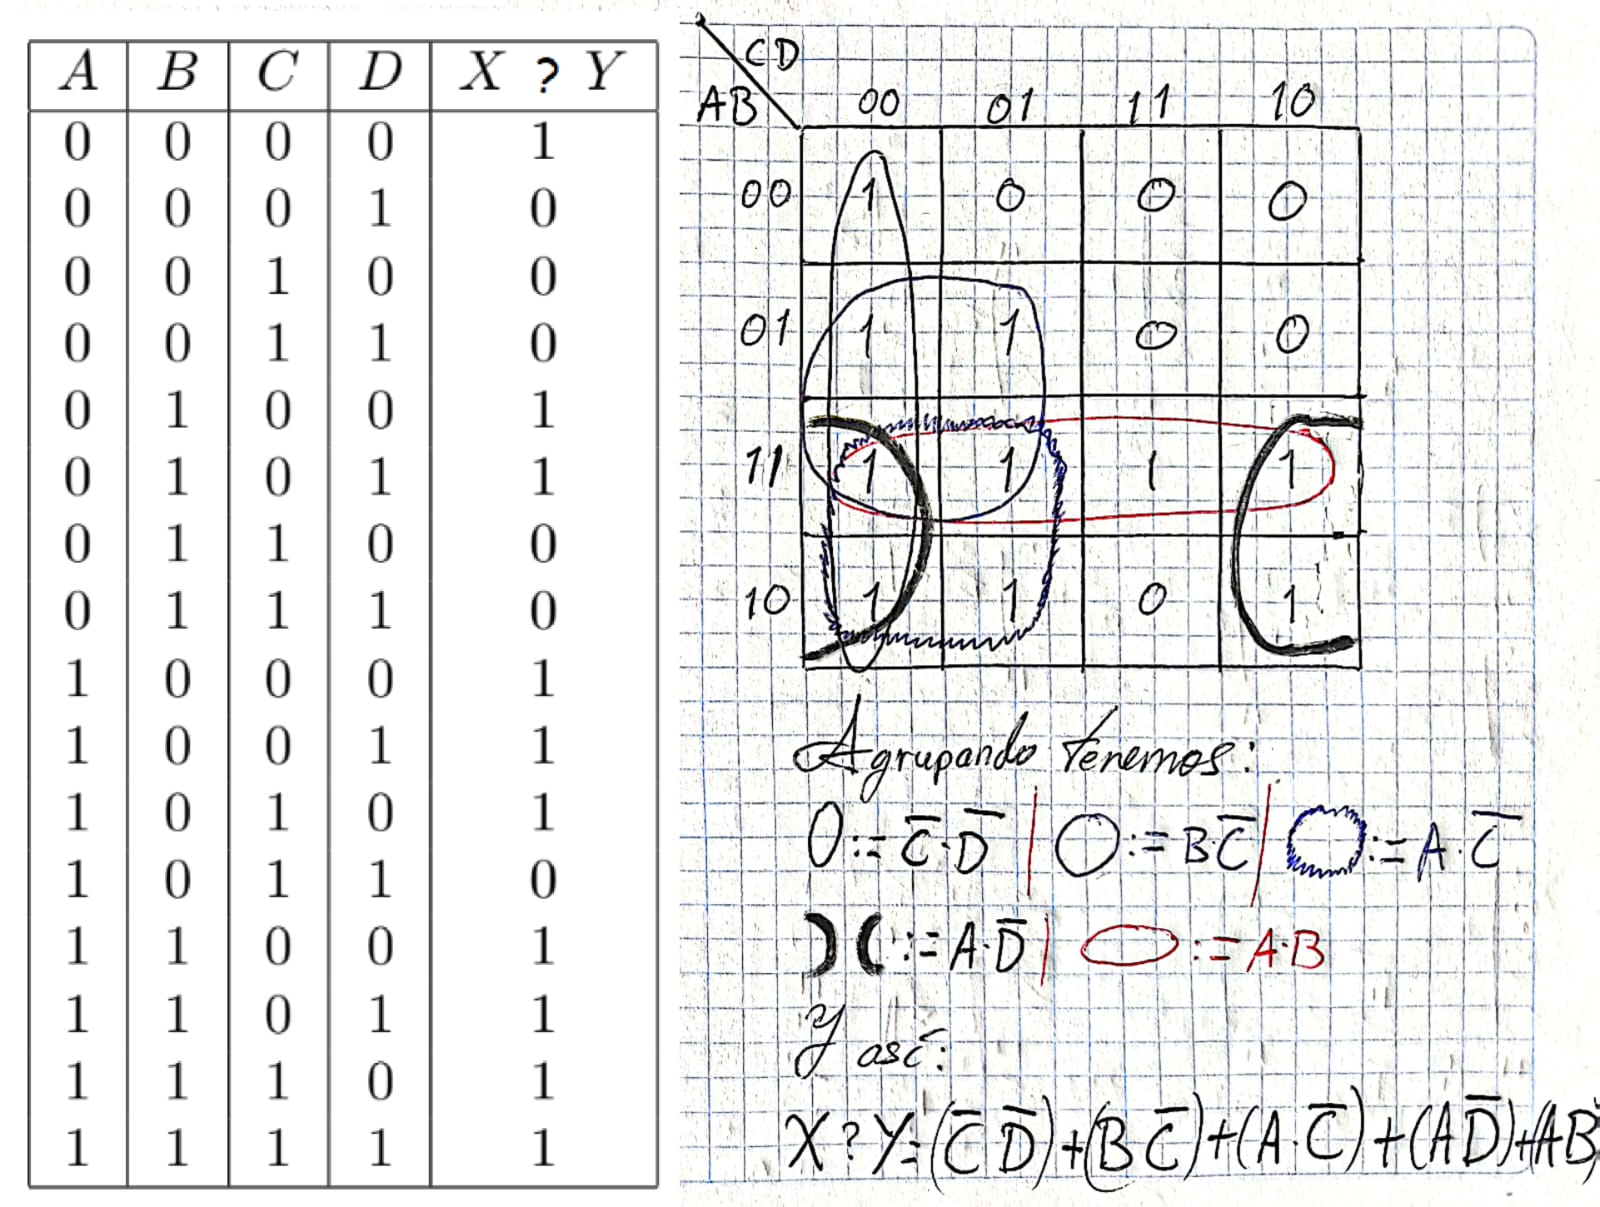
\includegraphics[width=0.5\textwidth]{ejercicio.png}
  \end{figure}
  
  El circuito implementa la funci\'{o}n $X \geq Y =$ (\={C}\={D}) + (B\={C}) + (A\={C}) + (A\={D}) + (AB), ya que tanto en la tabla, o en el mapa de Karnaugh con la ecuaci\'{o}n algebraica, como en el mismo circuito se puede apreciar esta comparaci\'{o}n donde $A \geq C \geq B \geq D$.\\
  Esto se puede notar claramente pues cuanto tenemos las 4 variables con el mismo valor tenemos un 1 como resultado, pues son iguales. Por otro lado si unicamente tenemos en 1 a $C$ o $D$ o ambos al mismo tiempo, tenemos como resultado 0, ya que AB no es mayor a $CD$ en estos casos. Y por \'{u}ltimo si A est\'{a} en 1 no importa el valor de $C$ o $D$ pues A siempre ser\'{a} mayor a CD, es decir si $A = 1$, entonces $AB \geq CD (X \geq Y)$.
\end{itemize}

\bigskip

\section*{Preguntas.}

\begin{enumerate}
  \item ¿Cuál es la diferencia entre un transistor P y uno N? ¿Cuáles son las partes de un transistor?
    
    \bigskip
    % -- Respuesta -- %
    Los transistores N (NPN) y P (PNP) son transistores bipolares de unión que se diferencian en la polaridad de la corriente que los activa:

    \begin{itemize}
    \item \textbf{NPN:} Se activa con corriente positiva en la base y permite el flujo de corriente del colector al emisor. Es el tipo más común y se usa en amplificación, conmutación y alta frecuencia.
    \item \textbf{PNP:} Se activa con corriente negativa en la base y permite el flujo de corriente del emisor al colector. También se usa como amplificador o interruptor electrónico.
    \end{itemize}

    \begin{figure}[H]
      \centering
      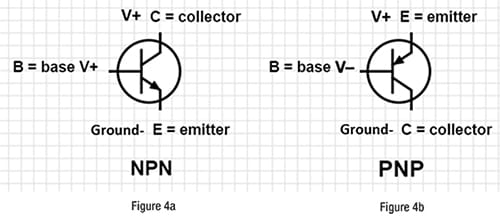
\includegraphics[width=0.5\textwidth]{transistores.png}
    \end{figure}
    
    Ambos funcionan de manera similar, pero requieren diferente polarización.
    Un transistor se conforma de tres partes:

    \begin{figure}[H]
      \centering
      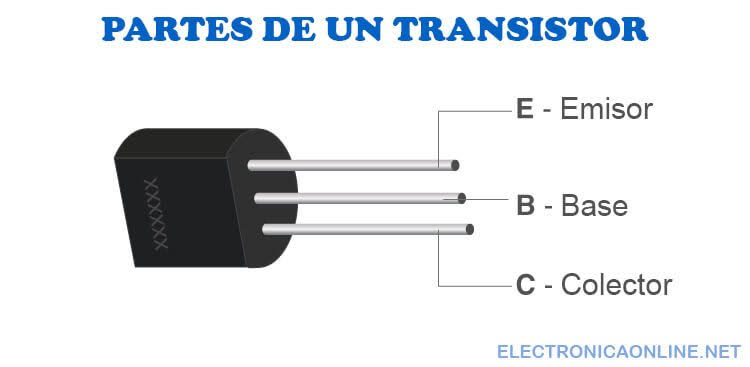
\includegraphics[width=0.5\textwidth]{transistor.png}
    \end{figure}
    
    \begin{itemize}
    \item \textbf{Base:} Controla el flujo de corriente entre el emisor y el colector.
    \item \textbf{Colector:} Recibe la corriente modulada.
    \item \textbf{Emisor:} Envía la corriente hacia el circuito.
    \end{itemize}
      
    Y este opera en tres estados:

    \begin{itemize}
    \item \textbf{Corte:} No conduce corriente (interruptor apagado).
    \item \textbf{Activa:} Conduce parcialmente (modulación de señal).
    \item \textbf{Saturación:} Conduce al máximo (interruptor encendido).
    \end{itemize}   

    Su funcionamiento se asemeja a una llave de paso de agua: si está cerrada, no fluye corriente; si está abierta, permite el paso parcial o total según la señal en la base. Esto permite su uso en amplificación y conmutación electrónica, fundamentales en circuitos lógicos y digitales.

    
  \item Teóricamente, ¿cuál es el tamaño más pequeño que un transistor puede tener? ¿Por qué es difícil hacer transistores mas pequeños?
    
    \bigskip
    % -- Respuesta -- %
    El tamaño mínimo teórico posible para un chip con la tecnología actual se conoce como el tamaño de la celda de transistor. Esta es una medida que se toma en nanómetros (nm). La celda de transistor estándar se fabrica actualmente con un tamaño de 5 nm, lo que significa que los transistores en el chip son de un tamaño de 5 nm. Sin embargo, hay algunas empresas que están trabajando en chips con transistores de tamaño de 2 nm.\\
    Pero el tamaño más pequeño alcanzado en laboratorio es 1 nm, desarrollado por el Laboratorio Berkeley en 2016. Sin embargo, la producción en masa aún no ha llegado a ese nivel. Actualmente, los transistores comerciales más pequeños son de 3 nm (fabricados por TSMC, Samsung y Apple), y para 2025 se espera avanzar en la producción de transistores de 2 nm (TSMC es la que los frabrica acutalmente).\\

    Reducir el tamaño de los transistores presenta desafíos físicos y tecnológicos:
    \begin{itemize}
    \item \textbf{Fenómenos cuánticos:} A escalas tan pequeñas, efectos como el túnel cuántico hacen que los electrones atraviesen barreras que antes los detenían, afectando el funcionamiento del transistor.
    \item \textbf{Límites materiales:} Los materiales tradicionales, como el silicio, dejan de ser eficientes, lo que obliga a investigar alternativas como el grafeno o los nanotubos de carbono.
    \item \textbf{Costos de fabricación:} La producción de transistores más pequeños requiere tecnología avanzada y costosa, dificultando su fabricación en masa.
    \end{itemize}   
    
  \item ¿Que tamaño tenían los transistores en 1975? ¿Y que tamaño tienen en el 2025? Usando la Ley de Moore, ¿cuándo llegaremos al transistor mas pequeño que nos dice la teoría.
    
    \bigskip
    % -- Respuesta -- %
    En 1975, los transistores tenían un tamaño de entre 5000 y 3000 nm.\\
    En 2025, empresas como TSMC han comenzado la producción de transistores de 2 nm.\\
    Según la Ley de Moore, el tamaño de los transistores se reduce aproximadamente a la mitad cada dos años. Siguiendo esta tendencia, podríamos ver transistores de 0.5 nm entre 2026 y 2027. Sin embargo, en los últimos años, la reducción del tamaño de los transistores ha desacelerado debido a limitaciones físicas como el túnel cuántico, lo que hace difícil mantener el ritmo predicho por la Ley de Moore.\\
    Intel estima que, en el futuro, los chips podrían contener 1 trillón de transistores, con tamaños cercanos a 0.5 nm, aunque esto dependerá de avances en nuevos materiales y tecnologías de fabricación.
    
  \item ¿Por qué se dice que los mapas de Karnaugh no nos dan una garantía de que siempre nos van a devolver la expresión mínima de la función?
    
    \bigskip
    % -- Respuesta -- %
    Los mapas de Karnaugh son una herramienta útil para simplificar expresiones booleanas, sin embargo, no siempre garantizan la expresión mínima absoluta, algunos factores que pueden influyen son:
    
    \begin{itemize}
    \item \textbf{Errores en la agrupación:}
      La minimización depende de la correcta agrupación de términos. Un error en la identificación de combinaciones óptimas puede llevar a una expresión subóptima.

    \item \textbf{Múltiples soluciones posibles:}
      Una misma función booleana puede tener varias formas mínimas equivalentes. Dependiendo de cómo se agrupen los términos, se pueden obtener diferentes expresiones, algunas más adecuadas que otras para la implementación en hardware.
      
    \item \textbf{No considera la implementación física:}
      Los K-maps reducen términos y variables, pero no optimizan necesariamente la cantidad de puertas lógicas necesarias ni la eficiencia del circuito. A veces, una expresión algebraicamente más simple puede requerir más hardware o ser más lenta.
      
    \item \textbf{Limitaciones con muchas variables:}
      Son prácticos hasta 6 variables (en teoría hasta 7, pero difíciles de manejar). Para funciones más grandes, métodos como \textit{Quine-McCluskey} o algoritmos computacionales como \textit{Espresso} suelen ser más eficientes.
    \end{itemize}
\end{enumerate}

\end{document}
